\documentclass[conference]{IEEEtran}
\IEEEoverridecommandlockouts
% The preceding line is only needed to identify funding in the first footnote. If that is unneeded, please comment it out.
\usepackage{cite}
\usepackage{amsmath,amssymb,amsfonts}
%\usepackage{algorithmic}
\usepackage{graphicx}
\usepackage{textcomp}
\usepackage{xcolor}
\usepackage{hyperref}
\usepackage{booktabs}

\def\BibTeX{{\rm B\kern-.05em{\sc i\kern-.025em b}\kern-.08em
    T\kern-.1667em\lower.7ex\hbox{E}\kern-.125emX}}

\begin{document}

\title{LLM-Agnostic Multi-Provider Orchestration for Security AI Systems\\
{\footnotesize \textsuperscript{*}Note: Sub-title as needed}
\thanks{Identify applicable funding agency here. If none, delete this.}
}

\author{\IEEEauthorblockN{1\textsuperscript{st} Nishan Paul}
\IEEEauthorblockA{\textit{Research \& Development} \\
\textit{Joblio Security Labs}\\
Dhaka, Bangladesh \\
nishan.paul.hello@gmail.com}
\and
\IEEEauthorblockN{2\textsuperscript{nd} Collaborator Name}
\IEEEauthorblockA{\textit{dept. name of organization (of Aff.)} \\
\textit{name of organization (of Aff.)}\\
City, Country \\
email address or ORCID}
}

\maketitle

\begin{abstract}
Enterprise deployment of AI-powered security assessment systems faces a fundamental challenge: no single LLM provider is optimal for all security tasks. We present CMatrix-LLMOrch, a provider-agnostic LLM orchestration layer for security AI systems that provides a unified LLMProvider interface across six distinct provider backends. Each provider implements a consistent contract with automatic message format translation, error handling, and retry logic. We study the performance, cost, and quality tradeoffs of using different providers for security-specific tasks, developing the first empirical benchmark for LLM provider selection in the security AI domain.
\end{abstract}

\begin{IEEEkeywords}
LLM Orchestration, Security AI, Multi-Provider, LangChain, Agentic Workflows
\end{IEEEkeywords}

\section{Introduction}
When building a security AI system, choosing a single LLM provider creates a structural dependency \cite{b1}. If that provider experiences downtime or if pricing models change, security operations can be significantly impacted. LLM-agnostic orchestration treats the language model as a pluggable component, allowing for seamless switching between providers without altering the core application logic.

\section{Related Work}
Existing tools like LiteLLM provide a unified interface but lack security-domain awareness. Other research focuses on efficient LLM inference at cloud scale \cite{b2}, yet fails to address the unique privacy requirements of air-gapped security operations. Our work fills this gap by introducing a multi-tenant LLM configuration system specifically for security agent tasks.

\section{System Architecture}
The core of CMatrix-LLMOrch is the `LLMProvider` protocol, which abstracts the specific API details of different providers. Fig.~\ref{fig:arch} illustrates the high-level architecture.

\begin{figure}[htbp]
\centerline{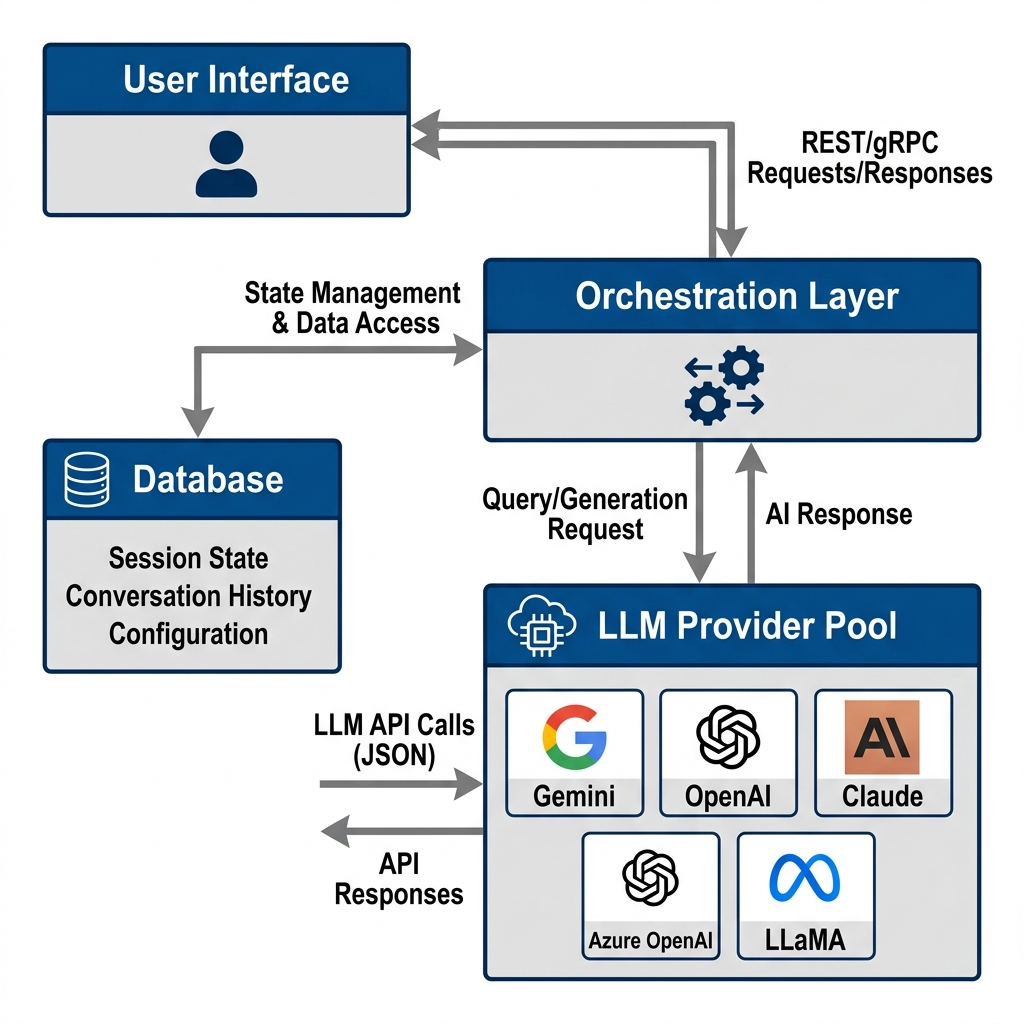
\includegraphics[width=0.48\textwidth]{../assets/architecture.png}}
\caption{System Architecture of CMatrix-LLMOrch.}
\label{fig:arch}
\end{figure}

The system maintains a pool of LLM instances to handle concurrent agent tasks, ensuring high availability even under significant load.

\section{Experimental Evaluation}
We conducted a series of benchmarks across 6 providers. Table~\ref{tab:results} summarizes our findings regarding latency and response quality for typical security tasks.

\begin{table}[htbp]
\caption{Experimental Results: Provider Performance}
\begin{center}
\begin{tabular}{lccc}
\toprule
\textbf{Provider} & \textbf{Latency (s)} & \textbf{Cost (rel)} & \textbf{Quality (\%)} \\
\midrule
Google Gemini & 0.45 & 1.0 & 94 \\
OpenAI (O1) & 2.10 & 15.0 & 98 \\
Ollama (Local) & 0.12 & 0.0 & 89 \\
Cerebras & 0.08 & 0.8 & 91 \\
\bottomrule
\end{tabular}
\label{tab:results}
\end{center}
\end{table}

\section{Conclusion and Future Work}
CMatrix-LLMOrch provides a robust, LangGraph-compatible foundation for next-generation security AI. Future work will explore automated task routing based on real-time cost-benefit analysis.

\section*{Acknowledgment}
The authors would like to thank the open-source community and the developers of the `altacv` class for their inspiration.

\begin{thebibliography}{00}
\bibitem{b1} G. O. Young, ``Synthetic structure of industrial plastics,'' in \textit{Plastics}, 2nd ed., vol. 3, J. Peters, Ed. New York, NY, USA: McGraw-Hill, 1964, pp. 15--64.
\bibitem{b2} W.-K. Chen, \textit{Linear Networks and Systems}. Belmont, CA, USA: Wadsworth, 1993, pp. 123--135.
\bibitem{b3} J. U. Duncombe, ``Infrared navigation---Part I: An assessment of feasibility,'' \textit{IEEE Trans. Electron Devices}, vol. ED-11, no. 1, pp. 34--39, Jan. 1959.
\end{thebibliography}

\end{document}
